\section{Intelligenza artificiale}

\subsection{Intelligenza artificiale}
I principali settori dell'IA sono:
\begin{itemize}
    \item Emulazione dei processi logici(conoscenza inserita dal progettista)
    \item Apprendimento automatico(Machine learning)
\end{itemize}

Le capacità richieste ad una IA sono:
\begin{itemize}
    \item Apprendere informazioni del mondo mediante un sistema di percezione(telecamere, dati, ecc)
    \item Dedurre sul mondo attraverso processi di inferenza
\end{itemize}

\subsubsection{Intelligenza artificiale e Intelligenza}
Con l'intelligenza artificiale si entra in un settore complicato, è difficile formulare una definizione di
Intelligente poichè spesso associato a umano, e tante altre domande di questo genere.

Visto che non sappiamo come funzioni l'intelligenza e la conoscenza,
per valutare una IA, si ricorre ad un test comportamentale.

\subsubsection{Test di Touring}
Un computer è da considerarsi intelligente
se, nell'interazione a distanza con un
essere umano, non è in grado di
distinguere se sta interagendo con un
uomo o una macchina.

Questa teoria spesso superata e riformulata, porta a definizione di AI debole(simula il pensiero) ed AI forte
(PENSA).

\subsubsection{AI: forte VS debole}
Non è comunemente accettato il fatto che la conoscenza umana possa essere replicata in una macchina
e altre idee simili.
\begin{itemize}
    \item le macchine pensano davvero o eseguono gli ordini?
    \item le macchine possono imparare a pensare?
    \item le macchine possono essere programmate per provare emozioni?
\end{itemize}

L'IA \textbf{forte} è una frma teorica per descrivere una certa mentalità dello sviluppo di sistemi AI.
Punta a creare intelligenze indistinguibili da quella umana.

In questo caso si potrebbe direr che la IA possa avere una coscienza(globalmente accettato?).

Secondo i fautori della IA \textbf{debole}, è impossibile attualmente creare una AI forte principalmente per la
assente definizione esplicita della intelligenza e comprensione.
I sostenitori della IA debole, affermano che una IA non debba avere una coscenza.


\begin{figure}[H]
    \centering
    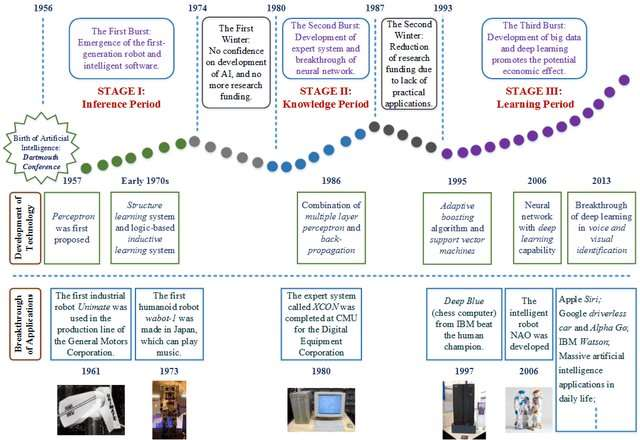
\includegraphics[width=1\linewidth]{imgs/11 - storia IA}
    \caption{Storia IA}
    \label{fig:storia_ia}
\end{figure}


